\documentclass[aspectratio=169,10pt]{beamer}
\usepackage[UTF8]{ctex}\usepackage{booktabs,tabularx,graphicx,amsmath}
\definecolor{navy}{HTML}{142B43}\definecolor{teal}{HTML}{168579}
\setbeamercolor{frametitle}{bg=navy,fg=white}\setbeamercolor{structure}{fg=teal}
\setbeamercolor{block title}{bg=teal,fg=white}\setbeamercolor{block body}{bg=teal!6}
\setbeamertemplate{navigation symbols}{}\setbeamerfont{frametitle}{size=\large}
\setbeamersize{text margin left=8mm,text margin right=8mm}
\setbeamertemplate{footline}{\leavevmode\hbox{\begin{beamercolorbox}[wd=.82\paperwidth,ht=2.5ex,dp=1ex,leftskip=1em]{author in head/foot}青序量化研究平台\quad Project 2 / RSRS\end{beamercolorbox}\begin{beamercolorbox}[wd=.18\paperwidth,ht=2.5ex,dp=1ex,center]{date in head/foot}\insertframenumber/16\end{beamercolorbox}}}
\begin{document}

\begin{frame}{RSRS：从研报到可核验实验}
\begin{block}{}复现核心结论，解释差异，检验一项风险改进\end{block}
\vspace{3mm}{\Huge\bfseries\color{navy}RSRS 择时研究}\par\vspace{3mm}
\small\begin{itemize}
\item Computational Finance · Project 2
\item 12412408 胡博文；12410819 谢明飞；12410436 王天希
\item 2026年10月19日 · 约15分钟
\end{itemize}
\end{frame}
\begin{frame}{研究问题与正式要求}
\begin{block}{}原文、实验、解释必须形成完整对应\end{block}
\small\begin{itemize}
\item 目标：2017年光大RSRS研报，图25、表5、图26
\item 先核公式和账本，再比较结果
\item 改进不奏效也保留；复用P1平台
\end{itemize}
\end{frame}
\begin{frame}{原文审计：暖机是关键发现}
\begin{block}{}原文早期使用部分历史，准备版等待完整窗口\end{block}
\small\begin{itemize}
\item 原文第22页：不足600个斜率时使用已有历史
\item 兼容实验与严格暖机实验分别展示
\item 样本首尾、成本和标准差细节未完全公开
\end{itemize}
\end{frame}
\begin{frame}{RSRS指标与交易状态}
\begin{block}{}滚动回归衡量高低价关系，阈值决定持仓状态\end{block}
\[z_t=\frac{\beta_t-\mu_{t-1,M}}{\sigma_{t-1,M}},\quad q_t=z_tR_t^2\beta_t\]
\small\begin{itemize}
\item H = \ensuremath{\alpha} + \ensuremath{\beta}L + \ensuremath{\varepsilon}；保留\ensuremath{\beta}及R\textsuperscript{2}
\item z \ensuremath{\to} zR\textsuperscript{2} \ensuremath{\to} zR\textsuperscript{2}\ensuremath{\beta}；右偏用N=16、M=300
\item 超过0.7入场，低于\ensuremath{-}0.7离场；MA只过滤入场
\end{itemize}
\end{frame}
\begin{frame}{信息时点与P1接入}
\begin{block}{}收盘形成目标，次日开盘成交，独立重建账户\end{block}
\small\begin{itemize}
\item 数据 \ensuremath{\to} RSRS指标/状态/权重 \ensuremath{\to} P1成交引擎
\item 次日开盘、每边10bp、现金0利息、无杠杆
\item 手算、未来扰动、账本和独立实现交叉核验
\end{itemize}
\end{frame}
\begin{frame}{三层样本分别回答不同问题}
\begin{block}{}兼容原样本、共同区间、发表后检验分开呈现\end{block}
\small\begin{itemize}
\item 原样本兼容：2005-03至2017-04，部分历史暖机
\item 共同区间：2007-08-01至2017-03-31，严格暖机
\item 发表后：2017-05-02至2026-10-15，已观察历史
\end{itemize}
\end{frame}
\begin{frame}{图25：同主题，并排看差异}
\begin{block}{}原文曲线与兼容实验连同假设一起比较\end{block}
\begin{center}\begin{minipage}[t]{.49\textwidth}\centering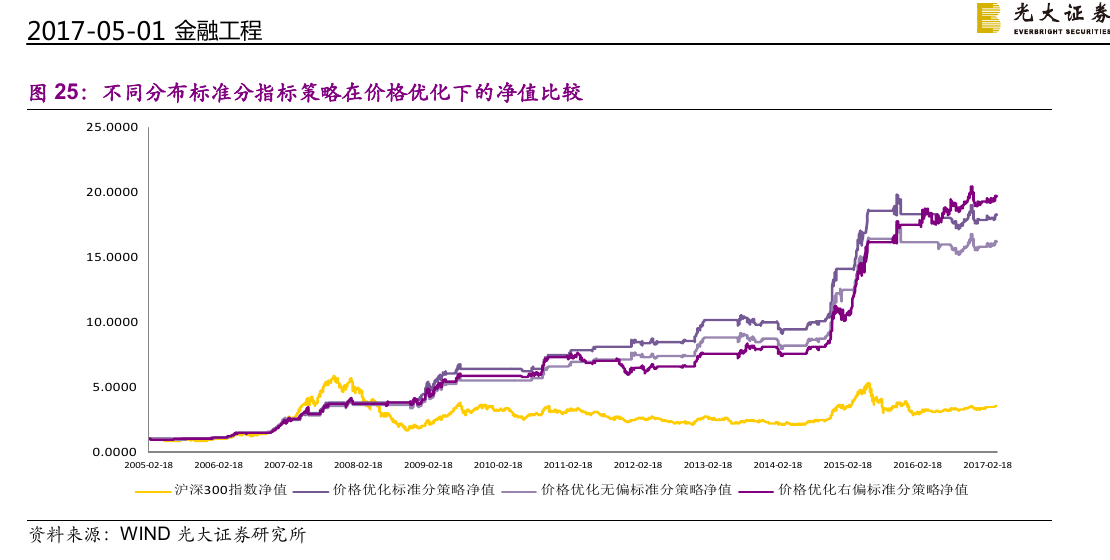
\includegraphics[width=\linewidth,height=44mm,keepaspectratio]{figures/source_figure25.png}\end{minipage}\hfill\begin{minipage}[t]{.49\textwidth}\centering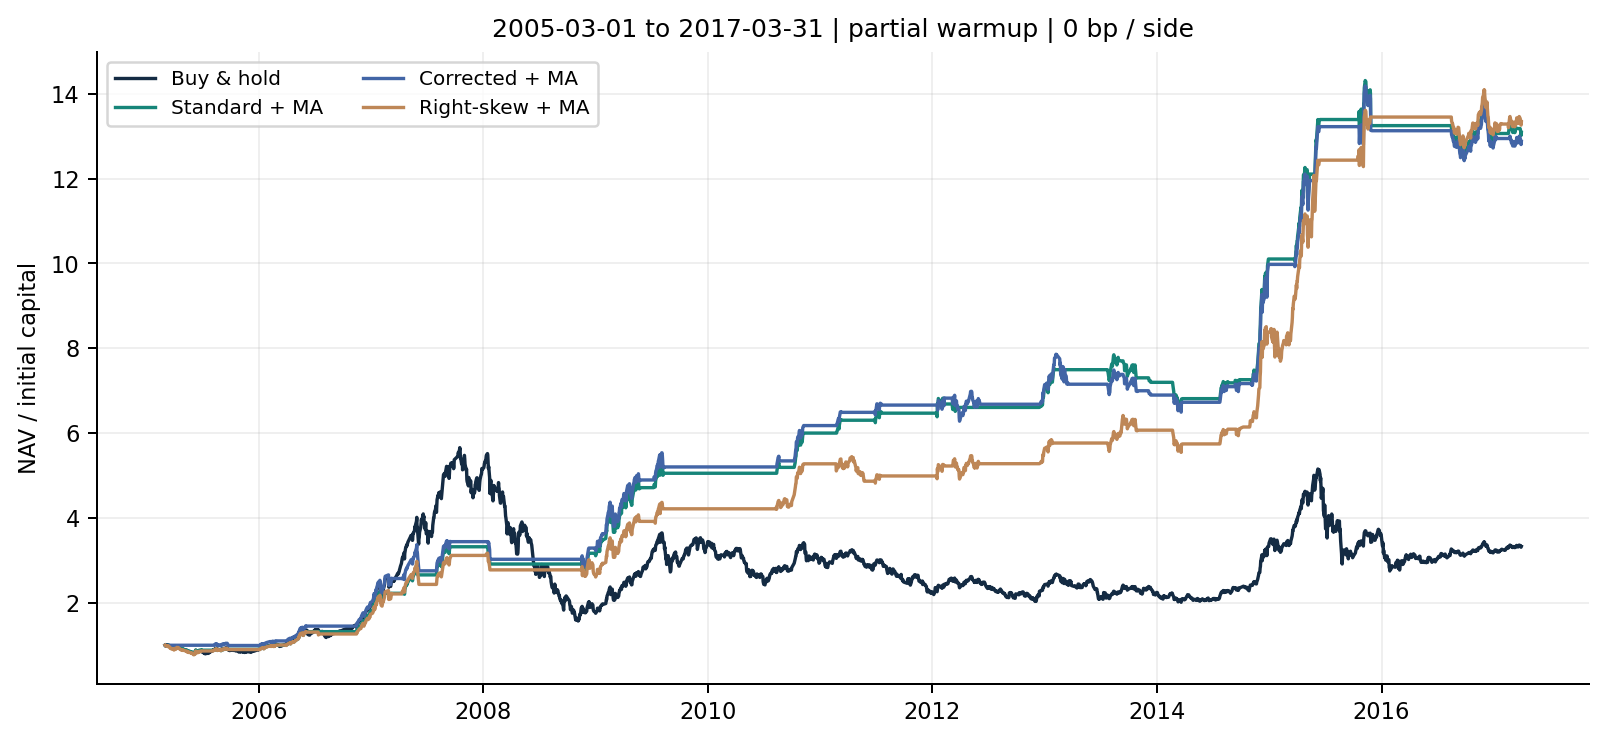
\includegraphics[width=\linewidth,height=44mm,keepaspectratio]{figures/reproduction_curves.png}\end{minipage}\end{center}
\small\begin{itemize}
\item 左：原文图25；右：本次部分窗口、零成本、次日开盘
\item 三类信号全部保留；不按最终收益选赢家
\end{itemize}
\end{frame}
\begin{frame}{表5：数字接近之前，先对齐定义}
\begin{block}{}原文年化28.19\%，不直接等于本次可比目标\end{block}
\begin{center}\scriptsize\begin{tabularx}{\textwidth}{Xrrr}\toprule
候选 & 原年化 & 本次年化 & 本次Sharpe\\\midrule
标准分+MA & 27.37\% & 24.65\% & 1.560\\
修正分+MA & 26.13\% & 24.48\% & 1.505\\
原右偏+MA & 28.19\% & 24.85\% & 1.404\\
\bottomrule\end{tabularx}\end{center}
\small\begin{itemize}
\item 原右偏+MA：年化28.19\%、Sharpe 1.56、回撤22.31\%
\item 本次年化/Sharpe/回撤统一定义，原表保留
\end{itemize}
\end{frame}
\begin{frame}{图26与控制实验：解释差异}
\begin{block}{}一次只改变一个主要因素，保留完整结果\end{block}
\begin{center}\begin{minipage}[t]{.49\textwidth}\centering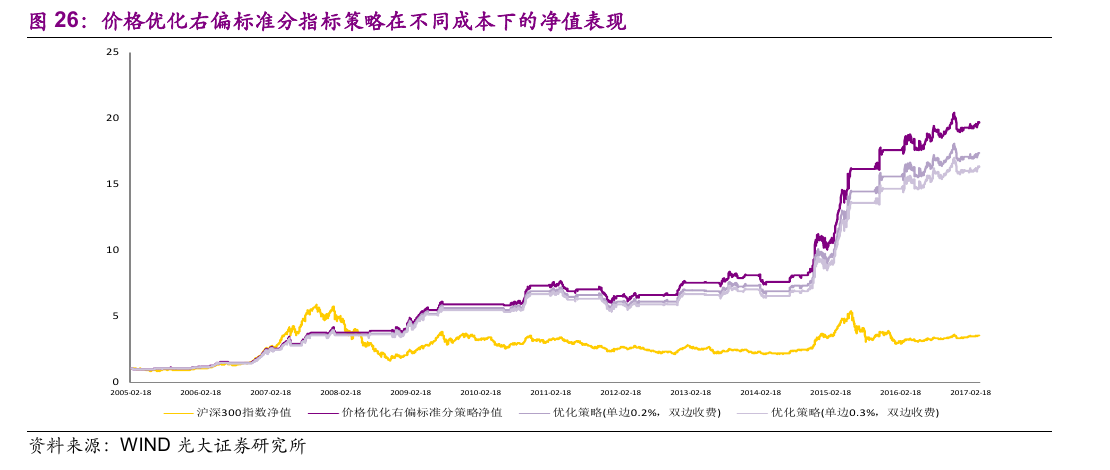
\includegraphics[width=\linewidth,height=44mm,keepaspectratio]{figures/source_figure26.png}\end{minipage}\hfill\begin{minipage}[t]{.49\textwidth}\centering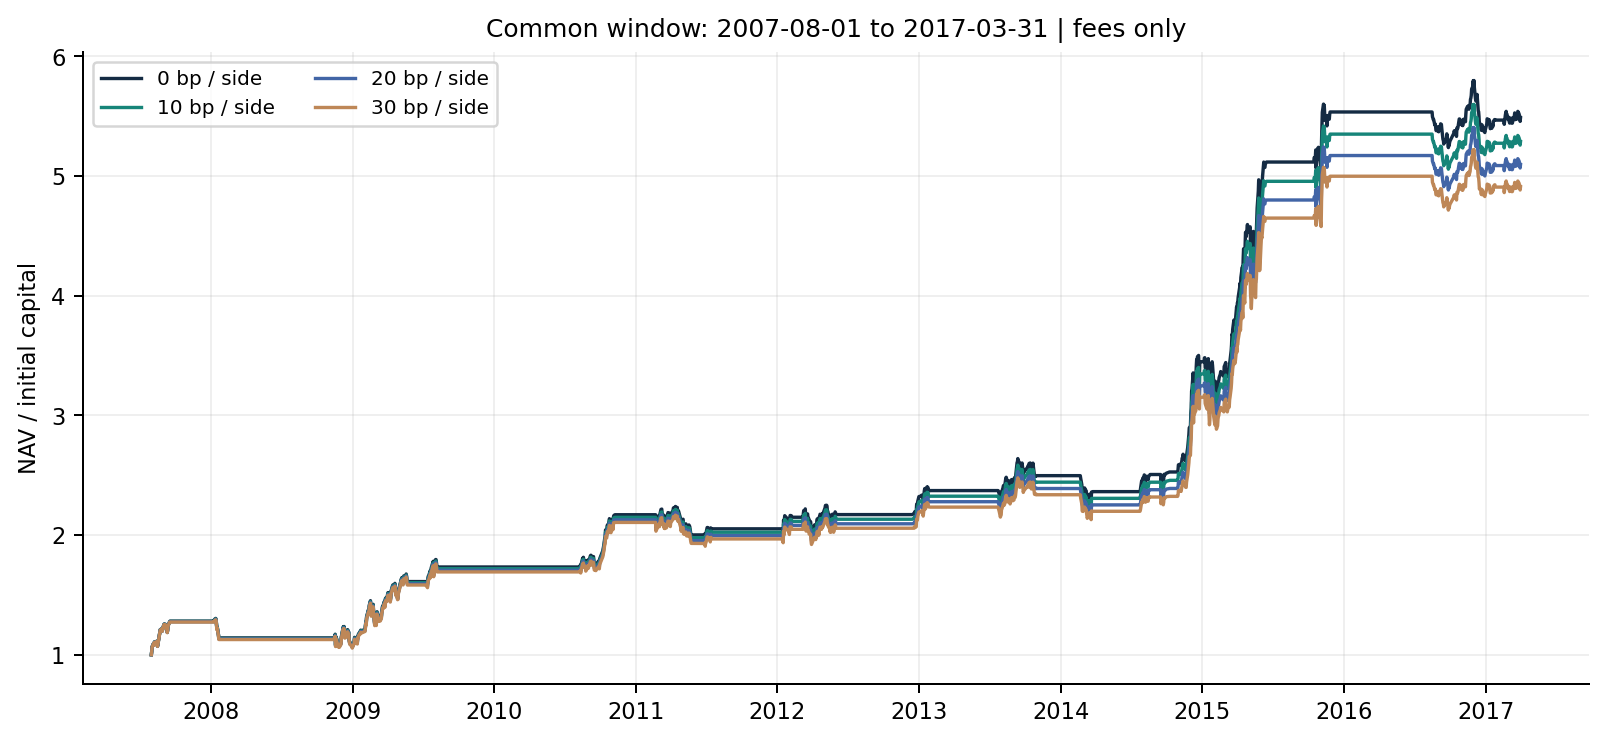
\includegraphics[width=\linewidth,height=44mm,keepaspectratio]{figures/cost_curves.png}\end{minipage}\end{center}
\small\begin{itemize}
\item 共同区间成本0/10/20/30bp，样本与原图不同
\item 收盘t信号，比较次日开盘与次日收盘成交
\end{itemize}
\end{frame}
\begin{frame}{自主改进：15\%波动率目标}
\begin{block}{}保留原信号，以过去20日波动决定投入比例\end{block}
\[w_t=s_t\min\!\left(1,\frac{0.15}{\sqrt{252}\,s(r_{t-19:t})}\right)\]
\small\begin{itemize}
\item w = 原信号 × min(1, 15\% / 估计年化波动)
\item 次日开盘每日调整；现金允许、上限100\%
\item 固定75\%仓位对照：检查是否只是少冒风险
\end{itemize}
\end{frame}
\begin{frame}{主结果：收益、风险与简单减仓一起看}
\begin{block}{}相对原策略：回撤-2.16pp；CAGR+0.32pp\end{block}
\begin{center}\scriptsize\begin{tabularx}{\textwidth}{Xrrr}\toprule
策略 & CAGR & Sharpe & 回撤\\\midrule
原右偏+MA & 1.50\% & 0.179 & 35.01\%\\
固定75\%仓位 & 1.30\% & 0.180 & 27.31\%\\
15\%波动目标 & 1.83\% & 0.227 & 32.85\%\\
买入持有 & 2.15\% & 0.207 & 45.60\%\\
\bottomrule\end{tabularx}\end{center}
\small\begin{itemize}
\item 原策略：CAGR 1.50\%，回撤 35.01\%
\item 15\%目标：CAGR 1.83\%，回撤 32.85\%
\end{itemize}
\end{frame}
\begin{frame}{稳健性与不确定性}
\begin{block}{}跨指数、费用与区块重采样检查依赖条件\end{block}
\begin{center}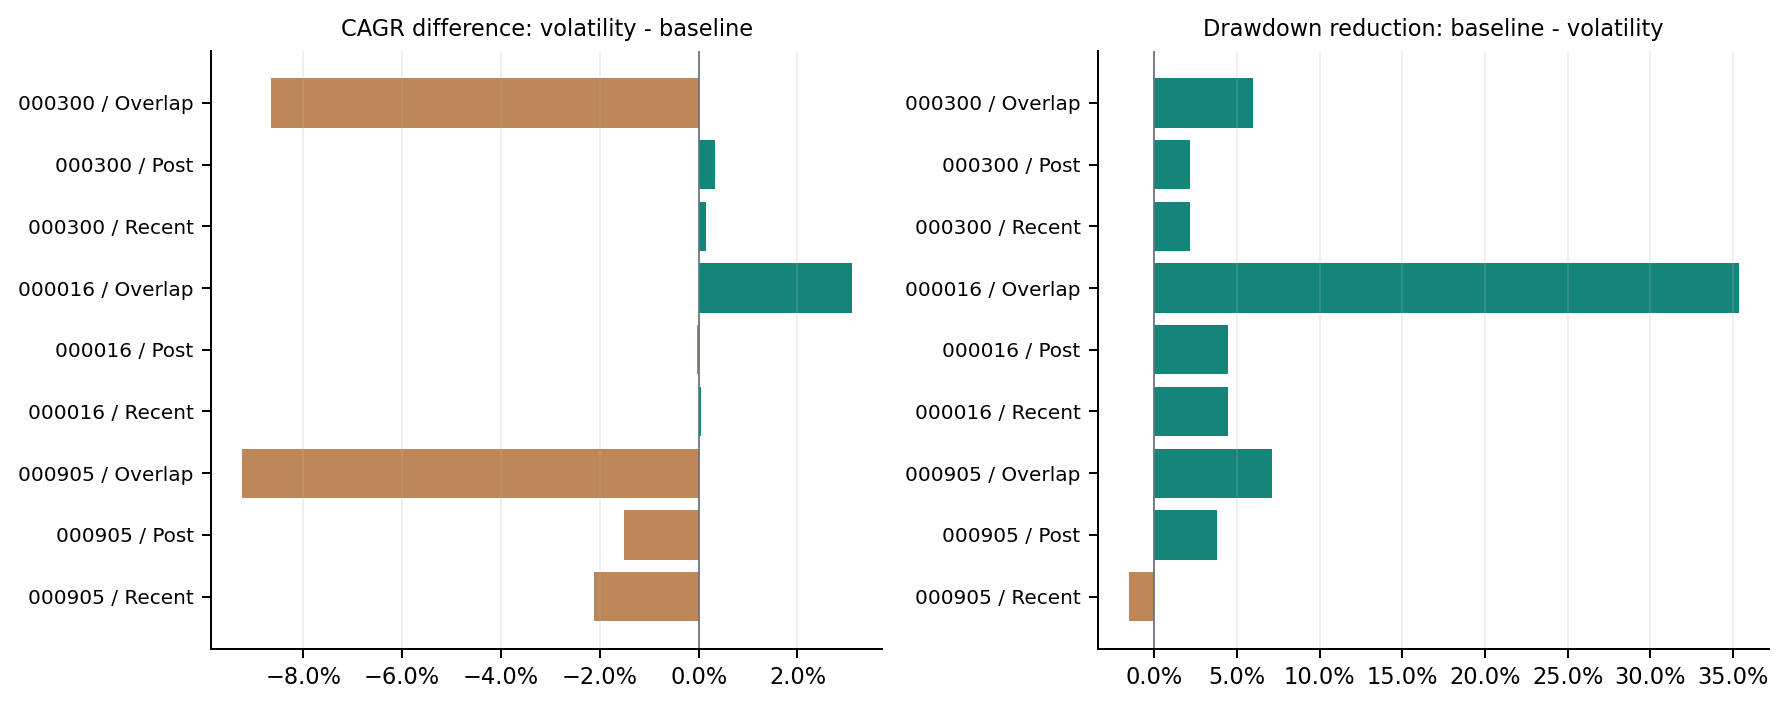
\includegraphics[width=.96\textwidth,height=43mm,keepaspectratio]{figures/robustness.png}\end{center}
\small\begin{itemize}
\item 三个指数 × 三个阶段；近期与发表后重叠
\item 10\%/15\%/20\%只作敏感性，不再选赢家
\end{itemize}
\end{frame}
\begin{frame}{平台演示与可复现交付}
\begin{block}{}同一界面查看原文、配置、结果和核验\end{block}
\small\begin{itemize}
\item 打开P2研究页，切换三层样本与策略
\item 检查信号、账本、成本和对照结果
\item 导出配置/证据；报告、Beamer、PPTX与讲稿对应
\end{itemize}
\end{frame}
\begin{frame}{结论：可解释的复现，比单条漂亮曲线更完整}
\begin{block}{}实现可核验，差异有对照，改进保留代价\end{block}
\small\begin{itemize}
\item 发现并量化原文部分历史暖机的影响
\item 固定信号加入风险仓位，并检验简单减仓替代
\item 下一步：真实ETF执行与冻结后的新数据
\end{itemize}
\end{frame}
\begin{frame}{备份：手算与指标口径}
\begin{block}{}可从三个观测点验证回归，再核对日账本\end{block}
\small\begin{itemize}
\item L=(1,2,3)，H=(2,3,5)：\ensuremath{\beta}=1.5，\ensuremath{\alpha}=1/3，R\textsuperscript{2}=27/28
\item 此前\ensuremath{\beta}=(1,2,3)，当前\ensuremath{\beta}=4：z=\ensuremath{\surd}6
\item Sharpe：252日年化、日收益样本标准差、rf=0
\end{itemize}
\end{frame}
\begin{frame}{备份：限制与复现实务}
\begin{block}{}没有把未知细节、历史复核或指数代理包装成确定性\end{block}
\small\begin{itemize}
\item Wind原始输入和作者精确样本未公开
\item 指数点位\ensuremath{\ne}可直接交易ETF；分红与冲击未建模
\item RSRS相关自动测试56项通过、0项跳过
\item 6项界面自动测试通过；正式页面策略切换、图表与下载已通过浏览器检查，57交易日回放核账通过
\end{itemize}
\end{frame}
\end{document}